\chapter{Research questions and Methodology}
% Methodology:
% - How do we answer RQs: simulation, controlled experiments, etc.

In this work we concentrate on the Change detection control unit (Figure~\ref{fig:fig3_gama_survey_cd}) which makes a decision when to retrain the model.
Implementation is done in a form of change detection algorithm.

Concept drifts are usually assumed to be not predictable.
We consider the case when they are predictable.



\begin{itemize}
  \item [i)] Model
  \item [ii)] Model with DDM
  \item [iii)] Model with DDM and embedded Pccf
\end{itemize}

Is it so that iii) is better than ii) and ii) is better than i) under certain assumptions?
If assumptions are wrong then even ii) is not better than i)~\cite{SouzaRMB20}.

In ~\cite{XXX} we demonstrated hhow FA arte and detection delays can be lowered for changedetection problem.
It can be used for concept drift handling in on-line learning under certain assumptions.


Figure~\ref{fig:research_question} illustrates the research question.
\begin{figure}[htb!]
	\centering
	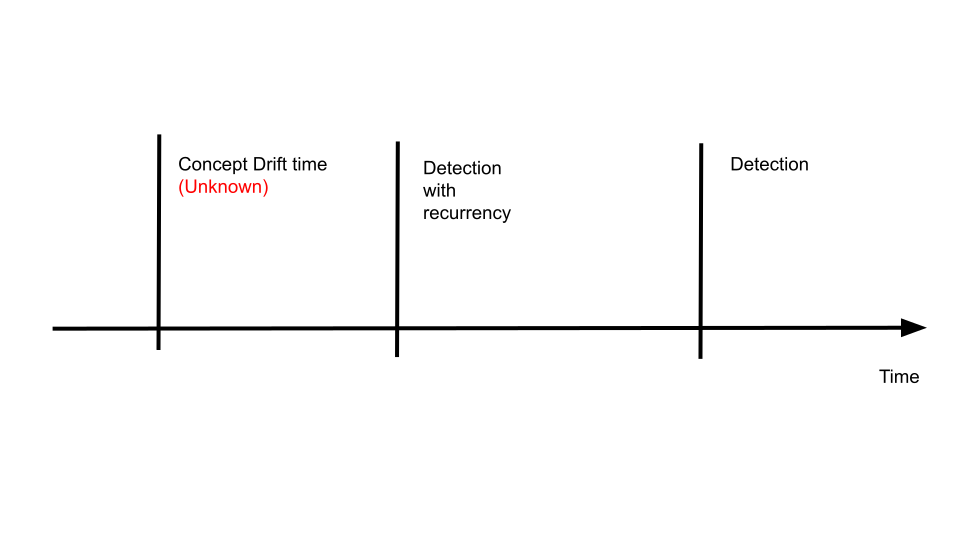
\includegraphics[width=0.9\textwidth]{images/google_slides/scheme_cd_recurrency}
  \caption{
	}\label{fig:research_question}
\end{figure}
